% ****** Start of file apssamp.tex ******
%
%   This file is part of the APS files in the REVTeX 4.1 distribution.
%   Version 4.1r of REVTeX, August 2010
%
%   Copyright (c) 2009, 2010 The American Physical Society.
%
%   See the REVTeX 4 README file for restrictions and more information.
%
% TeX'ing this file requires that you have AMS-LaTeX 2.0 installed
% as well as the rest of the prerequisites for REVTeX 4.1
%
% See the REVTeX 4 README file
% It also requires running BibTeX. The commands are as follows:
%
%  1)  latex apssamp.tex
%  2)  bibtex apssamp
%  3)  latex apssamp.tex
%  4)  latex apssamp.tex
%
\documentclass[%
 reprint,
%superscriptaddress,
%groupedaddress,
%unsortedaddress,
%runinaddress,
%frontmatterverbose, 
%preprint,
%showpacs,preprintnumbers,
%nofootinbib,
%nobibnotes,
%bibnotes,
 amsmath,amssymb,
 aps,
%pra,
%prb,
%rmp,
%prstab,
%prstper,
%floatfix,
]{revtex4-1}

\usepackage{graphicx}% Include figure files
\usepackage{subfigure}
\usepackage{multirow}
\usepackage{array}
\usepackage{dcolumn}% Align table columns on decimal point
\usepackage{bm}% bold math
%\usepackage{hyperref}% add hypertext capabilities
%\usepackage[mathlines]{lineno}% Enable numbering of text and display math
%\linenumbers\relax % Commence numbering lines

%\usepackage[showframe,%Uncomment any one of the following lines to test 
%%scale=0.7, marginratio={1:1, 2:3}, ignoreall,% default settings
%%text={7in,10in},centering,
%%margin=1.5in,
%%total={6.5in,8.75in}, top=1.2in, left=0.9in, includefoot,
%%height=10in,a5paper,hmargin={3cm,0.8in},
%]{geometry}

\usepackage{xeCJK}
%\setCJKmainfont[ItalicFont={KaiTi}, BoldFont={KaiTi}]{KaiTi}
\usepackage{textcomp}
\usepackage{chemfig}
\usepackage[version=4]{mhchem}
\usepackage{fontspec}
\usepackage{listings}
\usepackage{xcolor}
\usepackage{xcolor} % 定制颜色
\definecolor{mygreen}{rgb}{0,0.6,0}
\definecolor{mygray}{rgb}{0.5,0.5,0.5}
\definecolor{mymauve}{rgb}{0.58,0,0.82}
\lstset{
backgroundcolor=\color{white},      % choose the background color
basicstyle=\footnotesize\ttfamily,  % size of fonts used for the code
columns=fullflexible,
tabsize=4,
breaklines=true,               % automatic line breaking only at whitespace
captionpos=b,                  % sets the caption-position to bottom
commentstyle=\color{mygreen},  % comment style
escapeinside={\%*}{*)},        % if you want to add LaTeX within your code
keywordstyle=\color{blue},     % keyword style
stringstyle=\color{mymauve}\ttfamily,  % string literal style
frame=single,
rulesepcolor=\color{red!20!green!20!blue!20},
% identifierstyle=\color{red},
language=Mathematica,
}

\usepackage[normalem]{ulem}

\usepackage{tikz}
\usepackage{circuitikz}

\newcommand{\chuhao}{\fontsize{42pt}{44.9pt}\selectfont}    % 初号, 1.5倍行距
\newcommand{\xiaochu}{\fontsize{30pt}{40pt}\selectfont}    % 小初, 1.5倍行距
\newcommand{\yihao}{\fontsize{26pt}{36pt}\selectfont}    % 一号, 1.4倍行距
\newcommand{\erhao}{\fontsize{22pt}{28pt}\selectfont}    % 二号, 1.25倍行距
\newcommand{\xiaoer}{\fontsize{18pt}{18pt}\selectfont}    % 小二, 单倍行距
\newcommand{\sanhao}{\fontsize{16pt}{24pt}\selectfont}    % 三号, 1.5倍行距
\newcommand{\xiaosan}{\fontsize{15pt}{22pt}\selectfont}    % 小三, 1.5倍行距
\newcommand{\sihao}{\fontsize{14pt}{21pt}\selectfont}    % 四号, 1.5倍行距
\newcommand{\sihaox}{\fontsize{14pt}{28pt}\selectfont}    % 四号, 1.5倍行距
\newcommand{\banxiaosi}{\fontsize{13pt}{19.5pt}\selectfont}    % 半小四, 1.5倍行距
\newcommand{\xiaosix}{\fontsize{12pt}{24pt}\selectfont} 	% 小四, 1.5倍行距
\newcommand{\xiaosi}{\fontsize{12pt}{18pt}\selectfont}     
\newcommand{\dawuhao}{\fontsize{11pt}{11pt}\selectfont}    % 大五号, 单倍行距
\newcommand{\wuhao}{\fontsize{10.5pt}{10.5pt}\selectfont}    % 五号, 单倍行距
\newcommand{\xiaowu}{\fontsize{9pt}{9pt}\selectfont}    % 五号, 单倍行距

%\usepackage[fntef]{ctexcap}
%\CTEXsetup[number={\chinese{section}、},format={\Large\bfseries}]{section}
%\setCJKfamilyfont{fangsong}{FangSong}                      %仿宋2312 fs  
%\newcommand{\fangsong}{\CJKfamily{fangsong}}  

\usepackage{wrapfig}
\usepackage{fancyhdr}
\usepackage{fancybox}   






\newcommand{\bra}[1]{\langle #1 |}
\newcommand{\ket}[1]{| #1 \rangle}
\newcommand{\bracket}[2]{\langle #1 | #2 \rangle}
\newcommand{\bracketl}[3]{\langle #1 | #2 | #3 \rangle}
\newcommand{\func}{\mathrm \,}
\newcommand{\define}[2]{
	\begin{definition}
	\begin{description}
	\item[#1]
	#2
	\end{description}
	\end{definition}
}

\newcommand{\sch}{Schr\"odinger}
\newcommand{\grad}{\nabla}
\newcommand{\ueq}{\neq}
\newcommand{\celsius}{\ensuremath{^\circ\hspace{-0.09em}\mathrm{C}}}
\newcommand{\unit}[2]{$#1 \, \mathrm{#2}$}

\begin{document}

%\preprint{APS/123-QED}

\title{Measurement of conductivity of potassium chloride solution and critical micelle concentration of sodium dodecyl sulfate}% Force line breaks with \\
%\thanks{A footnote to the article title}% give thanks

\author{Rui Li}
 %\altaffiliation[Also at ]{Physics Department, XYZ University.}%Lines break automatically or can be forced with \\
%\author{Second Author}%
%\email{3160102098@zju.edu.cn}
\affiliation{%
 Qiushi science class (chemistry)\\
 Chu Kochen Honor College
}%

%\collaboration{MUSO Collaboration}%\noaffiliation

\author{Zong Wei Huang}
% \homepage{http://www.Second.institution.edu/~Charlie.Author}
%\affiliation{
% Second institution and/or address\\
% This line break forced% with \\
%}%
\affiliation{
Qiushi science class (chemistry)\\
 Chu Kochen Honor College
}%
%\author{Delta Author}
%\affiliation{%
% Authors' institution and/or address\\
% This line break forced with \textbackslash\textbackslash
%}%

%\collaboration{CLEO Collaboration}%\noaffiliation

%\date{\today}% It is always \today, today,
             %  but any date may be explicitly specified

\begin{abstract}
The infinite-dilute molar conductivity for potassium chloride solution as well as the critical micelle concentration of sodium dodecyl sulfate is obtained using Wheatstone bridge method. This measuring method is questioned according to the numerical analysis of the system using \emph{Mathematica}.
\begin{description}
\item[Keywords]
conductivity, potassium chloride, CMC, sodium dodecyl sulfate, Wheatstone bridge
\end{description}
\end{abstract}

%\pacs{Valid PACS appear here}% PACS, the Physics and Astronomy
                             % Classification Scheme.
%\keywords{Suggested keywords}%Use showkeys class option if keyword
                              %display desired
\maketitle

\tableofcontents

\section{Introduction}
Electrical resistivity is a fundamental property of a material that quantifies how strongly that material opposes the flow of electric current; while Electrical conductivity is defined as the reciprocal of electrical resistivity, and measures a material's ability to conduct an electric current. It is of great importance in electricity-involving activities, fuel cells being one of the examples.

Conductivity of a solution $G$ follows the following equation:
\begin{equation}
G = \kappa \frac{A}{l}
\end{equation}
where $A$ stands for the cross sectional area of the solution towards the flow of electricity, and $l$ for the length of it along the direction. $\kappa$ is a colligative constant that is determined for a certain substance or a solution.

Molar conductivity of a solution is defined as the conductivity of a solution containing 1 mol of the solvent,
\begin{equation}
\Lambda_m = \kappa / c
\end{equation}
For dilute solution of strong electrolytes, there is Kohlrausch law:
\begin{equation}
\Lambda_m = \Lambda^\infty_m - A \sqrt{c}
\end{equation}
which reveals linear relation between $\Lambda_m$ and $c$. Surfactants, however, presents a significant change of the slope $A$ at around a density, which is called 
critical micelle concentration (CMC). 

Wheatstone bridge is utilized to measure the electrical resistivity of the solution, thereby obtaining the molar conductivity of it. Alternating current is applied to avoid uneven concentration of solvents over the whole solution.

\section{Results and analysis}


\begin{figure}
\centering
\begin{circuitikz}
	\draw (6,0)
	to [V,v=$U$] (0,0);
	\draw (0,0)
	to [short] (0,4)
	to [C=$C$,i_=$I_2$] (1.5,3)
	to [R=$R_x$] (3,2)
	to [R=$R_3$] (6,4)
	to [short] (6,0);
	\draw (0,4)
	to [R=$R_1$,i_=$I_1$] (3,6)
	to [R=$R_2$] (6,4);
	\draw (3,6)
	to [ammeter,i_=$i$] (3,2);
	\end{circuitikz}
\caption{Electric circuit of the experiment, where $R_x$ stands for the electrical resistivity of the solution.}
\label{circuit}
\end{figure}


\begin{table}
\centering
\caption{Raw data of the measurement of conductivity of potassium chloride solution}
\begin{tabular}{cccc}\hline
$c$/M & $R_1/\Omega$ &$R_2/\Omega$ & $R_3/\Omega$ \\\hline 
 0.001250 & 2500 & 2000 & 1725.50 \\
  & 2500 & 3000 & 2611.00 \\
  & 2500 & 4000 & 3478.00 \\\hline
0.002500 & 2500 & 4000 & 2161.70 \\
			 & 2500 & 5000 & 2652.50 \\
			 &2500 & 3000 & 2611.00 \\\hline
 0.005000 & 2500 & 5000 & 1413.40 \\
			 & 2500 & 6000 & 1700.70 \\
 			& 2500 & 7000 & 1952.50 \\\hline
0.01000 & 2500 & 7000 & 1127.40 \\
 				& 2500 & 8000 & 1290.80 \\
				 & 2500 & 9000 & 1410.30 \\\hline
 0.02000 & 2500 & 2500 & 215.00 \\
  & 2500 & 5000 & 431.21 \\
  & 2500 & 10000 & 861.00 \\\hline
\end{tabular}
\label{kcldata}
\end{table}

\begin{table}
\centering
\caption{Raw data of the measurement of CMC of sodium dodecyl sulfate}
\begin{tabular}{cccc}\hline
$c/\mathrm{M}$ & $R_1/\Omega$ &$R_2/\Omega$ & $R_3/\Omega$ \\\hline 
 0.005000 & 2500 & 2500 & 2124.60 \\
 		 & 2500 & 3500 & 2975.80 \\
 		 & 2500 & 4500 & 3836.90 \\\hline
 0.007000 & 2500 & 2500 & 1655.50 \\
 		 & 2500 & 3500 & 2307.40 \\
 		 & 2500 & 5500 & 3701.00 \\\hline
 0.007500 & 2500 & 2500 & 1624.30 \\
 		 & 2500 & 3500 & 2259.30 \\
 		 & 2500 & 4500 & 2910.80 \\\hline
 0.008000 & 2500 & 2500 & 1565.00 \\
 		 & 2500 & 3500 & 2259.30 \\
 		 & 2500 & 4500 & 2762.00 \\\hline
 0.008500 & 2500 & 2500 & 1506.20 \\
 		 & 2500 & 3500 & 2098.00 \\
 		 & 2500 & 4500 & 2710.25 \\\hline
 0.009000 & 2500 & 2500 & 1413.13 \\
 		 & 2500 & 3500 & 1970.73 \\
 		 & 2500 & 4500 & 2503.75 \\\hline
 0.01000 & 2500 & 3000 & 1541.45 \\
 		 & 2500 & 4000 & 2060.05 \\
 		 & 2500 & 5000 & 2560.30 \\\hline
 0.01300 & 2500 & 3000 & 1309.80 \\
 		 & 2500 & 3000 & 1325.00 \\
 		 & 2500 & 4000 & 1766.50 \\
 		 & 2500 & 5000 & 2177.50 \\\hline
 0.01500 & 2500 & 5000 & 2020.00 \\
 		 & 2500 & 6000 & 2400.20 \\
 		 & 2500 & 8000 & 3217.40 \\\hline
\end{tabular}
\label{CMCdata}
\end{table}

The data from the experiment are shown in Table.\ref{kcldata},\ref{CMCdata}. The circuit adopted is represented by Fig.\ref{circuit} with the symbols given. Fig.\ref{KCL} shows graphic analysis of the data of the conductivity of potassium chloride solution, which shows strong inlinearity. The first data point contributes most to it, which might be attributed to contamination from the potassium chloride solution in high concentration. Excepting the first point, the line fitted is 
\begin{equation}
\Lambda_m = 0.01992- 0.04484\sqrt{c}
\end{equation}
which leads to the conclusion that $\Lambda_m^\infty = 0.01992 \, \mathrm{S\cdot m^2 \cdot mol^{-1}}$, with cell constant $K_\text{cell} = 59.53 \, \mathrm{m^{-1}}$.

Fig.\ref{CMC1} and Fig.\ref{CMC2} shows graphic analysis of the data of the conductivity of sodium dodecyl sulfate, with two linearly fitted lines from two separated datasets which have marked in the legends. Different slopes are conspicuous of two lines, nonetheless non-linearity is also apparent. The solutions for the intersection are $0.007660 \, \mathrm{M}$ and $0.009804 \, \mathrm{M}$ representing CMC, which present quite different results. 

\begin{figure}
\centering
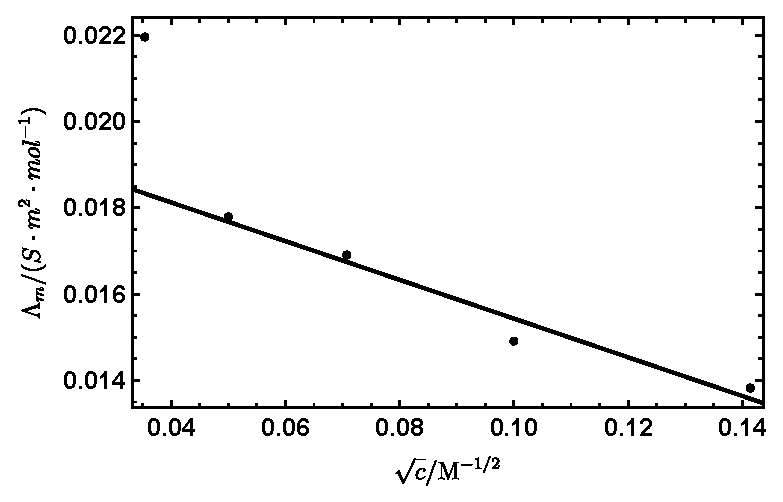
\includegraphics[width=0.45\textwidth]{figures/kcl.eps}
\caption{$\Lambda_m -\sqrt{c}$ data plots with its linear model fit}
\label{KCL}
\end{figure}

\begin{figure}
\centering
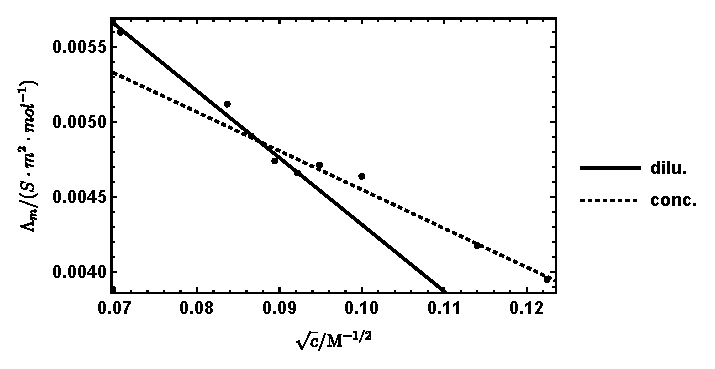
\includegraphics[width=0.45\textwidth]{figures/CMC1.eps}
\caption{$\Lambda_m - \sqrt{c}$ data plots with its linear model fits}
\label{CMC1}
\end{figure}

\begin{figure}
\centering
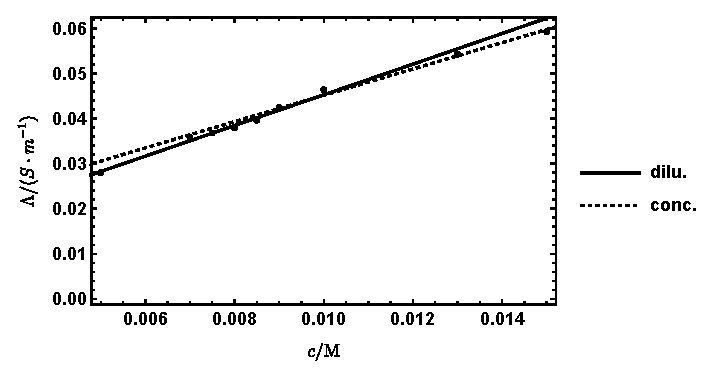
\includegraphics[width=0.45\textwidth]{figures/CMC2.eps}
\caption{$\Lambda - c$ data plots with its linear model fits}
\label{CMC2}
\end{figure}


\begin{figure}
\centering
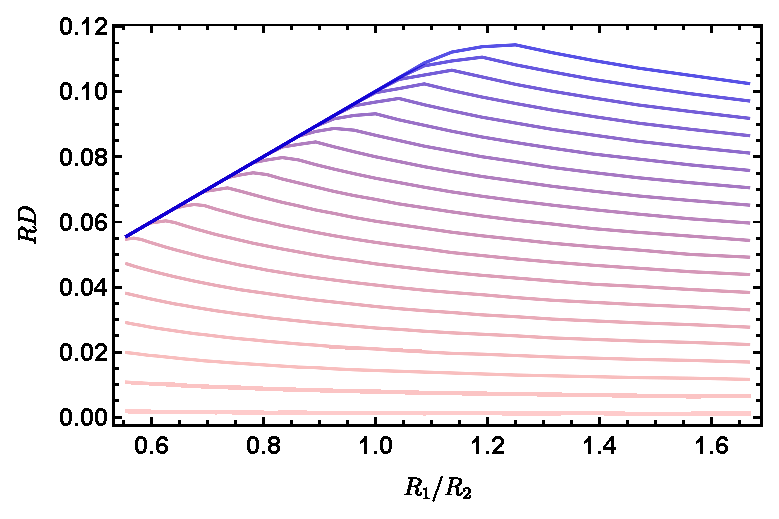
\includegraphics[width=0.45\textwidth]{figures/R1R2Ratio.eps}
\caption{The relative deviation of the $R_x$ calculated from possible $R_3$ sets compared with true $R_x$ value (1000 $\Omega$) \emph{v.s.} the amplifier($R_1/R_2$), setting $C$ to 1 F. Different lines represent different minimum detectable current of the current detector varying from $10^{-6}\sim10^{-4}$~A, with each line representing minimum current $5 \times 10^{-6}$~A higher than beneath.}
\label{R1R2Ratio}
\end{figure}

\begin{figure}
\centering
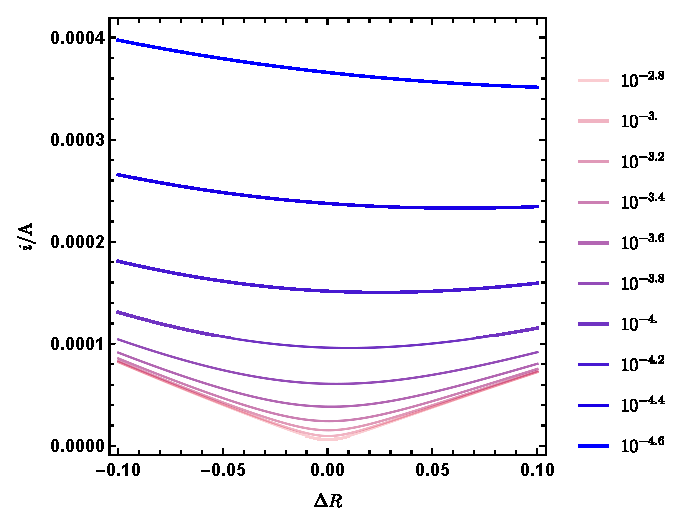
\includegraphics[width=0.45\textwidth]{figures/ideltaRcurve.eps}
\caption{The current that flows through the current detector \emph{v.s.} the relative deviation of $R_3$ from $R_x$, with $R_1/R_2$~set to 1, at different values of $C$ which have been listed in the legends with the unit F.}
\label{idelta}
\end{figure}

there might exist a huge error in both experiments, which stems from the insensibility of the current detector in the electric bridge system. To further elaborate it, a differential equation system is deduced,
\begin{equation}
\begin{cases}
I_1 R_1 +(I_1 -i) R_2 = U_0 \sin{\omega t} \\
I_2 R_x + (I_2+i) R_3 = U_0 \sin{\omega t} - u \\
(I_1 -i) R_2 - i r - (I_2 + i) R_3 =0 \\
I_2 = C \frac{d u}{dt}
\end{cases}
\end{equation}
with each term represented in Fig.\ref{circuit}. The solution is considered as a series connection of a theoretical conductor and resistance, regardless of the electrochemical reaction. Such an assumption does not lead to a mich simpler form of the solution thus \emph{Mathematica} is utilized to give analytical solution with numerical sets of data, thanks to its superior symbolic calculating system:
\begin{lstlisting}
WheatstoneSolve = 
 DSolve[{I1[t] R1 + (I1[t] - i[t]) R2 == U0 Sin[w t], 
    I2[t] Rx + (I2[t] + i[t]) R3 == 
     U0 Sin[w t] - u[t], (I1[t] - i[t]) R2 - 
      i[t] r - (I2[t] + i[t]) R3 == 0} /. {I2[t] -> 
     c D[u[t], t]}, {I1[t], u[t], i[t]}, t]
\end{lstlisting}
and is packaged as a function:
\begin{lstlisting}
isolve = i[t] /. WheatstoneSolve;

relation[r1_, r2_, r3_, rx_, R_, u0_, q_, omega_] := 
  FindMaximum[
     isolve /. {w -> omega, U0 -> u0, R1 -> r1, R2 -> r2, R3 -> r3, 
       Rx -> rx, r -> R, C[1] -> 0, c -> q}, {t, 0}][[1]]/Sqrt[2];
\end{lstlisting}

Parameters are given as discrete sets of numerical data and manipulated by the packaged function,returning results:
\begin{lstlisting}
testlist = 
 Table[Table[{2500, 2500 + 100 a, (2500 + 100 a)/2500*1000 + b, 1000, 
    100, 8, q, 50}, {a, -10, 20}, {b, -100, 100, 0.2}], {q, 0.1, 1, 
   0.1}]

relation @@@ Flatten[testlist, 2]

ratiosentivitymatrix = 
  Table[Transpose[{Table[2500/(
      2500 + 100 a), {a, -10, 
       20}], (Partition[
           Length /@ (Select[#, # < q*10^-6 &] & /@ 
              Partition[simulationdata, 1001]), 31][[1]]/10/1000)*
      Table[2500/(2500 + 100 a), {a, -10, 20}]}], {q, 1, 100, 5}];

testlist2 = 
 Table[Table[{2500, 2500 + 100 a, (2500 + 100 a)/2500*1000 + b, 1000, 
    100, 8, q/10^10, 50}, {a, -10, 20}, {b, -100, 100, 0.2}], {q, 0.1,
    1, 0.2}]

simulationdata2 = relation @@@ Flatten[testlist2, 2]

ratiosentivitymatrix2 = 
  Table[Table[
    Transpose[{Table[2500/(
       2500 + 100 a), {a, -10, 
        20}], (Partition[
            Length /@ (Select[#, # < q*10^-6 &] & /@ 
               Partition[simulationdata, 1001]), 31][[k]]/10/1000)*
       Table[2500/(2500 + 100 a), {a, -10, 20}]}], {q, 1, 100, 
     5}], {k, 1, 5}];

testlist3 = 
 Table[Table[{2500, 2500, 1000 + b, 1000, 100, 8, 10^(-q), 
    50}, {b, -100, 100, 0.2}], {q, 0, 10, 0.2}]

simulationdata3 = relation @@@ Flatten[testlist3, 1]
\end{lstlisting}
It needs to be stated that $R_1$~is set globally as 2500 $\Omega$, $R_x$~as 1000 $\Omega$,and $r$, resistance of the current detector, as 100 $\Omega$~in the test data sets,$U$ as 8 V, and $R_2$ changes on an 100 $\Omega$ basis around 2500 $\Omega$, while $R_3$~changes on an 0.2 $\Omega$ basis, which simulates the manipulations during the experiment, around $\frac{R_1R_2}{R_x}$, or `what it should be'. The function returns the current that flows through the current detector, or to be more specific,
\begin{equation}
i = \frac{i_\text{max}}{\sqrt{2}}
\end{equation}
according to the sinusoidal behavior of alternative currents.
 
The corresponding result data is manipulated according to the principle that a current under a certain number is regarded as `undetectable', and the corresponding $R_3$~sets are regarded as `optimized solutions' for the circuit equally. This gives Fig.\ref{R1R2Ratio}, which highlights the dependence of the choice of $R_1/R_2$, if the current detector is not sensitive enough. It also reveals the fact that increase of $R_1/R_2$ rather amplifies the error, if the sensitivity is relatively high, and it has the opposite trend in lower sensitivity of the current detector. In other words, it is only recommended to adopt lower $R_1/R_2$, or larger amplifier of $R_x$ towards $R_3$, only if the current detector is not sensitive enough, at a level of $10^{-5}$~A.

Fig.\ref{idelta} reveals the dependence of the equivalent capacity of the solution, and that a solution having equivalent capacity larger than $10^{-3}$~F can completely ignore the effect of capacitator, and gives correct result of $R_x$, which is very hard to achieve. It means that system error might also arise from the capacity of the solution, even under alternative current. From the two figures the validity of the method is questioned.

\section{Conclusion}
The infinite-dilute molar conductivity for potassium chloride solution is deduced as $\Lambda_m^\infty = 0.01992 \, \mathrm{S\cdot m^2 \cdot mol^{-1}}$, while the CMC of sodium dodecyl sulfate is given as $0.007660 \, \mathrm{M}$ and $0.009804 \, \mathrm{M}$ using two methods. The measuring method is questioned according to great deviation of $R_x$ as well as inevitable system error that arises from the low capacity of the solution.


\section{Acknowledgement}
This report is greatly assisted by Zong Wei Huang, who provide enumerous help in furnishing the theoretical model of the system.

\end{document}

\begin{figure}
\centering
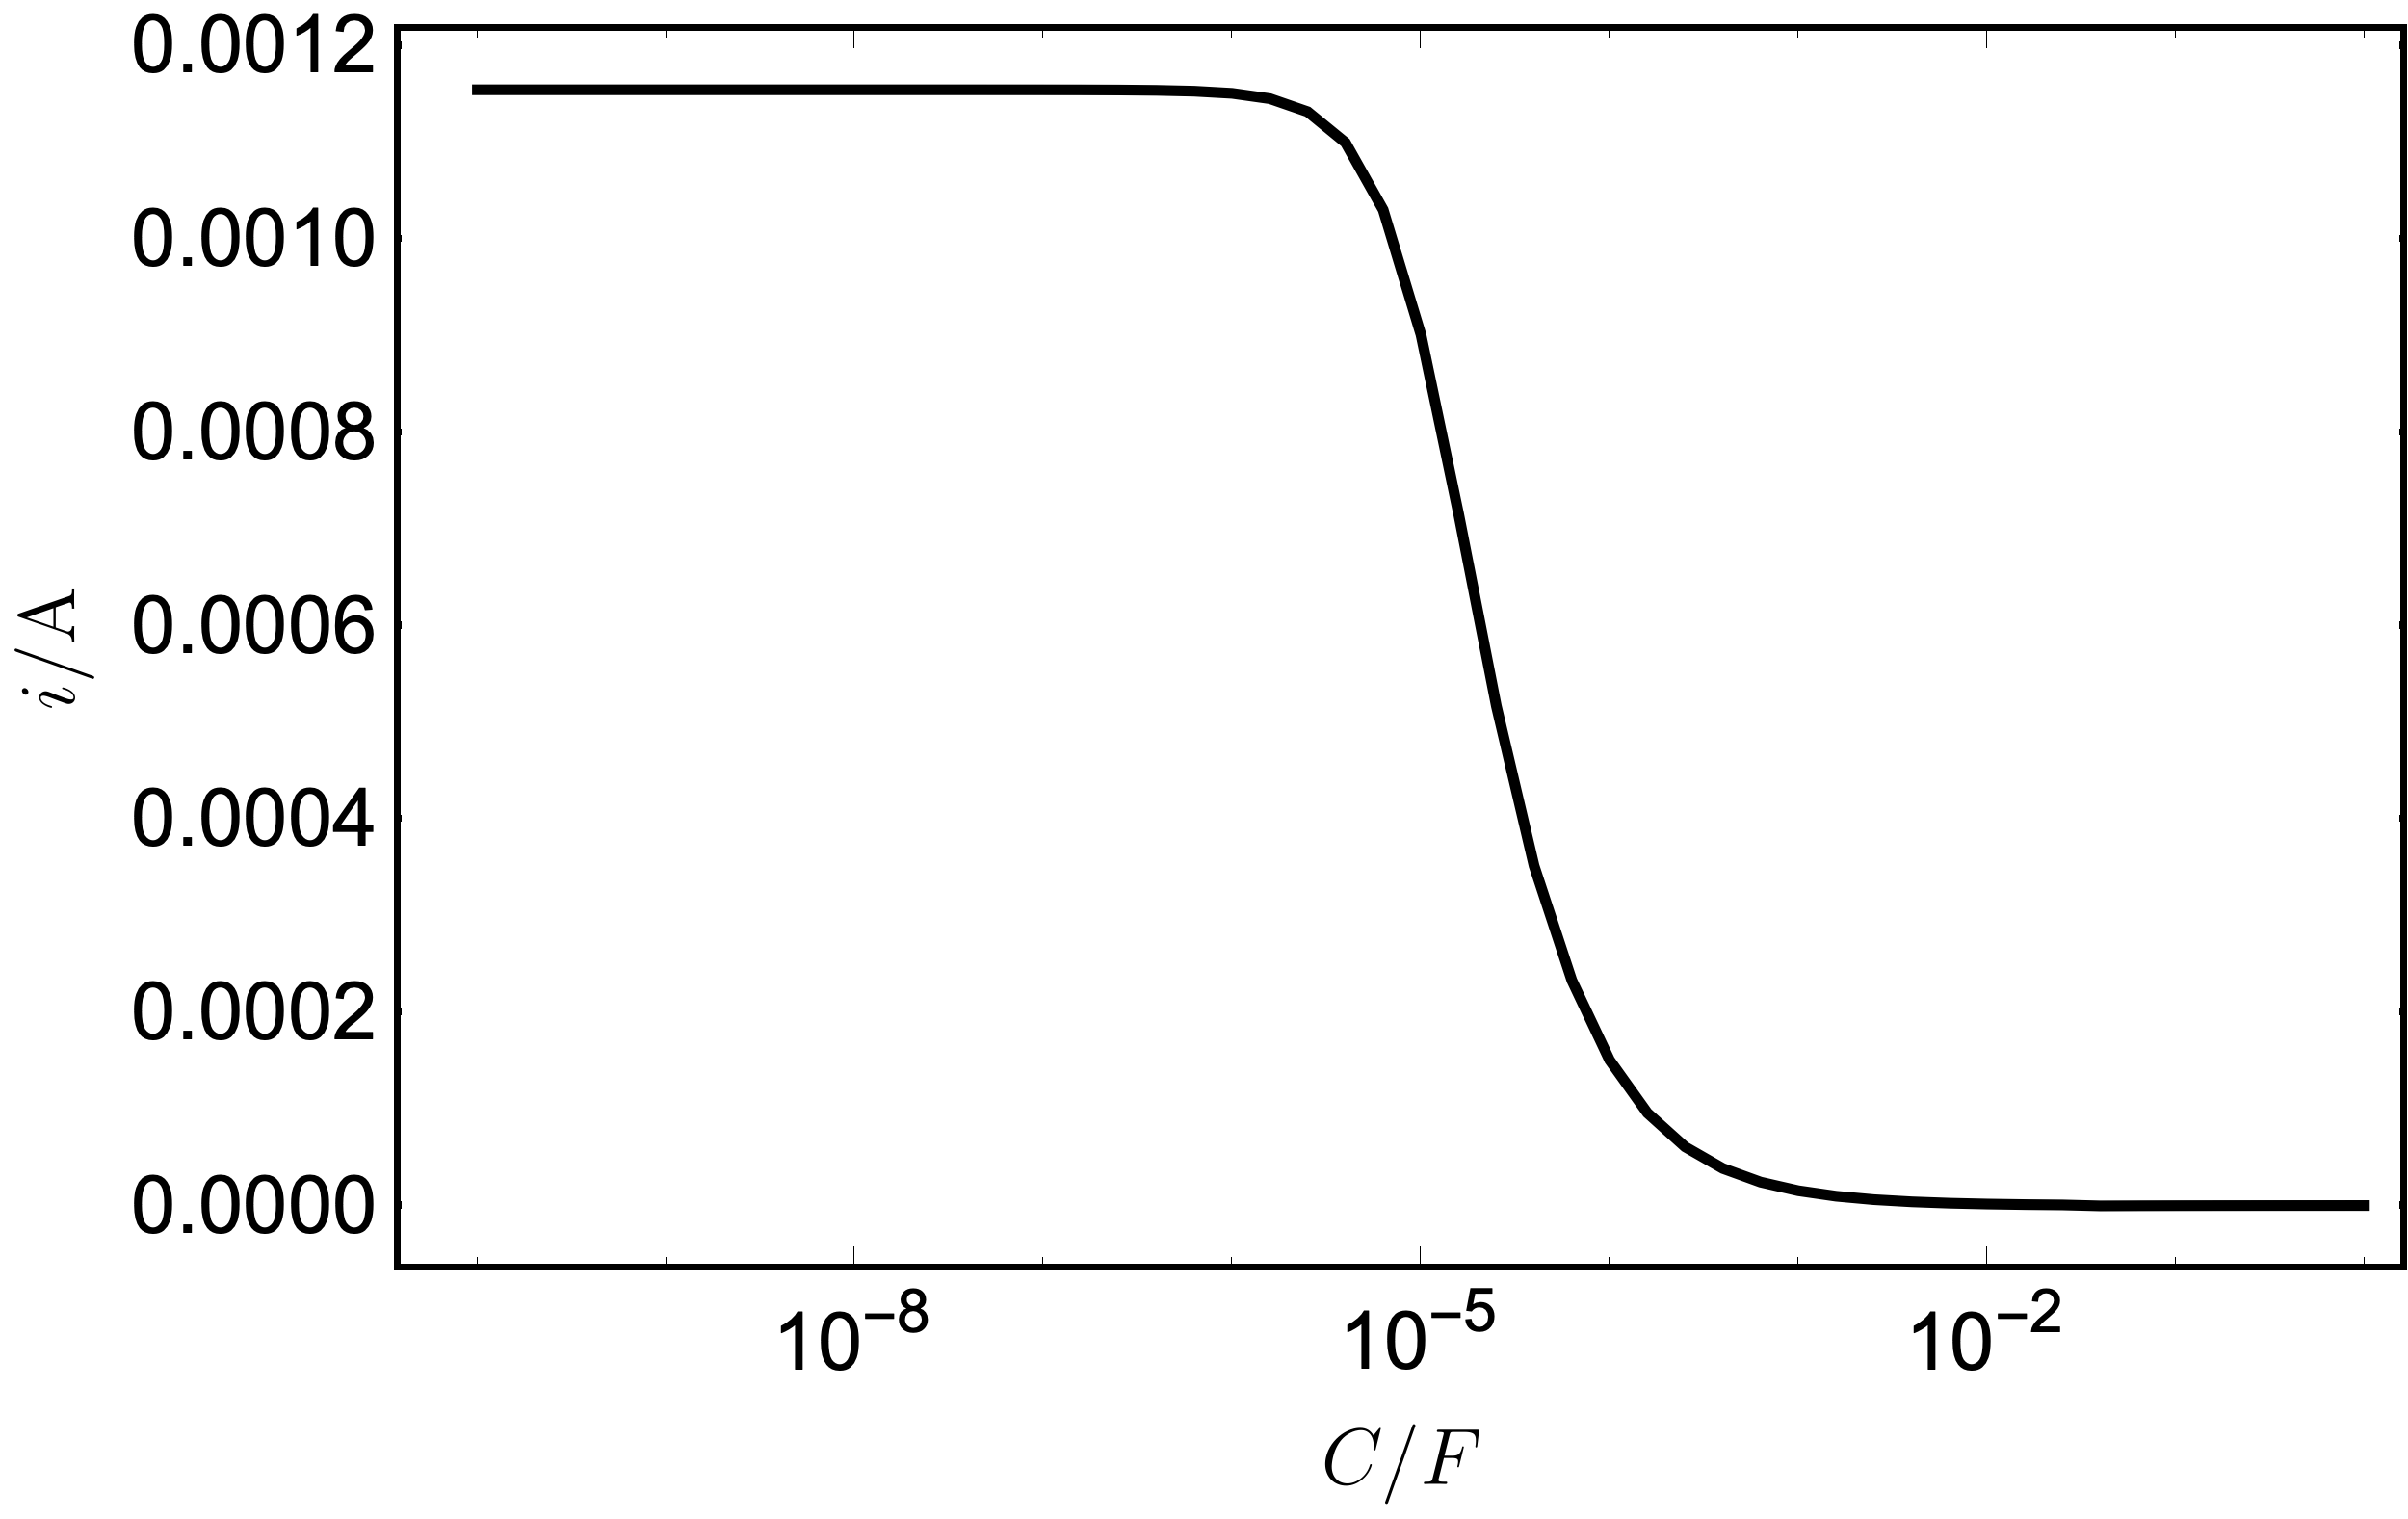
\includegraphics[width=0.45\textwidth]{figures/Ci.png}
\caption{The minimum current that flows through the current detector at a variation of $R_3$, \emph{v.s.} the different values of$C$. The $R_1/R_2$~ is set to 1 and $R_x$ to 1000 $\Omega$.}
\label{Ci}
\end{figure}
